\documentclass{article}
\usepackage[utf8]{inputenc}
\setlength{\parskip}{5pt} % esp. entre parrafos
\setlength{\parindent}{0pt} % esp. al inicio de un parrafo
\usepackage{listings} % listings
\usepackage{color} %colores
\usepackage{amsmath} % mates
\usepackage[sort&compress,numbers]{natbib} % referencias
\usepackage{url} % que las URLs se vean lindos
\usepackage[top=15mm,left=20mm,right=20mm,bottom=25mm]{geometry} % margenes
\usepackage{hyperref} % ligas de URLs
\usepackage{graphicx} % poner figuras
\usepackage[spanish,es-tabla]{babel} % nombre tablas
\usepackage{caption}
\usepackage{subcaption}



\definecolor{mypink}{rgb}{0.976, 0.462, 0.847}
\definecolor{mygray}{rgb}{0.976, 0.980, 0.980}
\definecolor{myblue}{rgb}{0.258, 0.682, 1}
\definecolor{mypink2}{rgb}{0.525, 0.054, 0.4}
\lstset{ 
  backgroundcolor=\color{mygray},
  commentstyle=\color{myblue},
  keywordstyle=\color{mypink}, 
  numberstyle=\tiny\color{mypink}
  stringstyle=\color{mypink2}, 
  breaklines=true,
}



\title{Tarea 11}
\author{Eduardo Navarro}
\date{Noviembre 2021}

\begin{document}

\maketitle

\section{Introducción}
En esta práctica se analizó el porcentaje de soluciones de Pareto en función del número de funciones objetivo. Después se analizaron los resultados obtenidos.

\section{Desarrollo}
Con las instrucciones de la tarea \cite{pareto} y lo visto en clase \cite{twitchsimu} se le hicieron modificaciones al código para obtener el porcentaje a determinados números de funciones. Se añadió un \texttt{for} para las funciones \texttt{"k"} dadas de 2, 3, 4 y 5 además de otro \texttt{for} para las repeticiones.

\begin{lstlisting} [language=R, caption= Código para la obtención del porcentaje de soluciones de Pareto a determinados números de funciones.] 
datos = data.frame()

vc <- 4
md <- 3
tc <- 5
ka <- c(2,3,4,5) # cuantas funciones objetivo
obj <- list()
je<- 1:50


for (k in ka) {
for (repe in je) {

for (i in 1:k) {
  obj[[i]] <- poli(md, vc, tc)
}

...

frente <- subset(val, no.dom) # solamente las no dominadas

porcentaje = (length(frente[,1])/n)*100



resultado = c(k, repe, porcentaje)
datos = rbind(datos, resultado)
names(datos) = c("k", "Replica", "Porcentaje")
}
}
\end{lstlisting}
 Con esto se generaron los datos de la tabla \ref{tabla1} y se procedió a graficar \ref{grafica1}.
 
 \begin{table}[h!]
\centering
\caption{Ejemplo de datos obtenidos.}
\label{tabla1}
\begin{tabular}{|c|r|r|}
\hline
\textbf{k} & \multicolumn{1}{c|}{\textbf{Réplica}} & \multicolumn{1}{c|}{\textbf{Porcentaje}} \\ \hline
2 & 1.0 & 0.5 \\ \hline
2 & 2.0 & 6.0 \\ \hline
2 & 3.0 & 3.5 \\ \hline
2 & 4.0 & 7.5 \\ \hline
2 & 5.0 & 5.0 \\ \hline
2 & 6.0 & 2.0 \\ \hline
2 & 7.0 & 2.5 \\ \hline
\end{tabular}
\end{table}

\begin{figure} [h!]% figura
\renewcommand{\figurename}{Gráfica}
    \centering
    \caption{ \% de soluciones a funciones dadas.}
    \label{grafica1}
    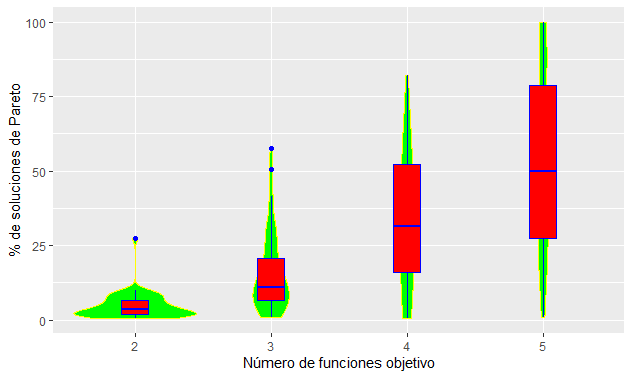
\includegraphics[width=150mm]{grafica1.png} % archivo
\end{figure}

\begin{lstlisting} [language=R, caption= Código para la obtención de la gráfica y análisis estadístico.]
library(ggplot2) # recordar instalar si hace falta

datos$k = as.factor(datos$k)
gr <- ggplot(datos, aes(x=k, y=Porcentaje)) + geom_violin(fill="green", color="yellow")
gr + geom_boxplot(width=0.2, fill="red", color="blue", lwd=0.5) +
  labs(x = "Numero de funciones objetivo", y = "% de soluciones Pareto")
  
library(tidyverse)

funcionporc<-datos%>%
  group_by(k) %>%
  summarise(
    
    promedio = mean(Porcentaje, na.rm = TRUE),
    desviacion_std = sd(Porcentaje, na.rm = TRUE),
    varianza = sd(Porcentaje, na.rm = TRUE)^2,
    mediana = median(Porcentaje, na.rm = TRUE),
    rango_intercuartil = IQR(Porcentaje, na.rm = TRUE)
  )

pshapiro<-tapply(datos$Porcentaje, datos$k, shapiro.test)

kruskal.test(Porcentaje~k, data=datos)

pwilcox<-pairwise.wilcox.test(datos$Porcentaje, datos$k)
\end{lstlisting}
De la gráfica \ref{grafica1} podemos ver que hay diferencias considerables conforme aumenta el número de funciones objetivo. Para comprobarlo se realizaron las pruebas de  Shapiro–Wilk \cite{shapiro} y Kruskal-Wallis \cite{Kruskall} junto con la prueba Wilcox \cite{pairwise} para el análisis de datos.

\begin{table}[h!]
\centering
\caption{Datos estadísticos obtenidos.}
\label{tabla2}
\begin{tabular}{|c|r|r|r|r|r|}
\hline
\textbf{k} & \multicolumn{1}{c|}{\textbf{Promedio}} & \multicolumn{1}{c|}{\textbf{Desviacion std}} & \multicolumn{1}{c|}{\textbf{Varianza}} & \multicolumn{1}{c|}{\textbf{Mediana}} & \multicolumn{1}{c|}{\textbf{Rango intercuartil}} \\ \hline
2 & 4.66 & 4.34 & 18.82 & 3.50 & 4.50 \\ \hline
3 & 15.57 & 12.96 & 168.00 & 11.00 & 14.25 \\ \hline
4 & 33.75 & 23.00 & 528.92 & 31.50 & 36.00 \\ \hline
5 & 53.90 & 31.36 & 983.48 & 49.75 & 51.38 \\ \hline
\end{tabular}
\end{table}

\begin{table}[h!]
\centering
\caption{Resultados de la prueba Shapiro–Wilk.}
\label{tabla3}
\begin{tabular}{|c|r|r|}
\hline
\textbf{Funciones} & \multicolumn{1}{c|}{\textbf{W}} & \multicolumn{1}{c|}{\textbf{P}} \\ \hline
2 & 0.7145 & $1.52\times 10^{-8}$ \\ \hline
3 & 0.8696 & $5.48\times 10^{-5}$ \\ \hline
4 & 0.9535 & 0.0474 \\ \hline
5 & 0.9234 & 0.0031 \\ \hline
\end{tabular}
\end{table}

\begin{table}[h!]
\centering
\caption{Resultados de la prueba Kruskal-Wallis.}
\label{tabla4}
\begin{tabular}{|c|c|}
\hline
\textbf{H(3)} & \textbf{P} \\ \hline
\multicolumn{1}{|r|}{99.15} & \multicolumn{1}{r|}{$2.20\times 10^{-16}$} \\ \hline
\end{tabular}
\end{table}

\begin{table}[h!]
\centering
\caption{Resultados de la prueba por parejas de Wilcox.}
\label{tabla5}
\begin{tabular}{|c|r|c|c|}
\hline
\textbf{Funciones} & \multicolumn{1}{c|}{\textbf{2}} & \textbf{3} & \textbf{4} \\ \hline
\textbf{3} & $5.60\times 10^{-8}$ & - & - \\ \hline
\textbf{4} & $4.40\times 10^{-10}$ & \multicolumn{1}{r|}{0.0001} & - \\ \hline
\textbf{5} & $8.50\times 10^{-15}$ & \multicolumn{1}{r|}{$7.30\times 10^{-10}$} & \multicolumn{1}{r|}{0.0014} \\ \hline
\end{tabular}
\end{table}

Para el reto 1 se utilizó el \texttt{kmeans} \cite{kmean} para el análisis del frente obtenido y separarlo a diversos porcentajes del mismo, obteniéndose las gráficas de la figura \ref{fig1} en dónde el rojo es el frente original y el verde es el subconjunto. 

\newpage

\begin{figure}[h!]
\centering
\caption{Frente a diversos porcentajes.}
\begin{subfigure}[b]{0.45\linewidth}
\includegraphics[width=\linewidth]{r130.png}
\caption{30\%}
\label{r130}
\end{subfigure}
\begin{subfigure}[b]{0.45\linewidth}
\includegraphics[width=\linewidth]{r140.png}
\caption{40\%}
\label{r140}
\end{subfigure}
\begin{subfigure}[b]{0.45\linewidth}
\includegraphics[width=\linewidth]{r170.png}
\caption{70\%}
\label{r170}
\end{subfigure}
\label{fig1}
\end{figure}

\begin{lstlisting} [language=R, caption= Código para la obtención de las gráficas del reto 1.]
porcentajes=70
res.k<-kmeans(frente, round(dim(frente)[1]*porcentajes/100), iter.max = 1000, nstart = 1000,
       algorithm = c("Hartigan-Wong", "Lloyd", "Forgy",
                     "MacQueen"), trace=FALSE)
tablas<-res.k$centers
res.k$betweenss / res.k$totss

png("p11_frentesub2.png", width=15, height=15, units="cm", res=1200)
plot(val[,1], val[,2], xlab=paste(xl, "mejor con cuadro azul"),
     ylab=paste(yl,"mejor con bolita naranja"),
     main=NULL)
points((tablas[,1]), (tablas[,2]), col="green", pch=16, cex=1.5)
points((frente[,1]), (frente[,2]), col="red", pch=16, cex=0.9)
mejor1 <- which.max((1 + (-2 * minim[1])) * val[,1])
mejor2 <- which.max((1 + (-2 * minim[2])) * val[,2])
points(val[mejor1, 1], val[mejor1, 2], col="blue", pch=15, cex=0.5)
points(val[mejor2, 1], val[mejor2, 2], col="orange", pch=16, cex=0.5)
graphics.off()
\end{lstlisting}

\section{Conclusiones}
De la práctica podemos concluir que mientras más funciones se tienen se alcanza un mayor rango de porcentaje de soluciones de Pareto. A un número de funciones bajas se concentra el \% de soluciones en la parte baja del rango intercuartil. Al aumentar el número de funciones se observa una concentración casi uniforme a lo largo del rango intercuartil. De las pruebas estadísticas de Shapiro–Wilk se tiene que no tienen una distribución normal pero se observa que esta aumenta conforme el número de funciones aumenta hasta cierto punto, luego vuelve a decrecer. De la prueba de Kruskal-Wallis se rechaza la hipótesis nula y se concluye que las medianas no son todas iguales y para observar mejor estas diferencias, de la prueba por parejas de Wilcox se observa como todos los grupos son significativamente diferentes. Se cree que el comportamiento se debe a que al haber más rutas dimensionales se pueden tener más soluciones óptimas y por ende puede aumentar el porcentaje. Del reto 1 se logró un subconjunto dependiente del porcentaje deseado.

\bibliography{referencias}
\bibliographystyle{plainnat}
\end{document}
